\documentclass[oneside,a4paper,12pt]{article} % Specifies the page format and font size.

% -------------------------------------- Integration of packages -------------------------------------- 
% Literature and language
	\usepackage[english]{babel}
	\usepackage[style=bwl-FU,backend=bibtex,natbib=true,maxcitenames=2]{biblatex}
	\addbibresource{Content/Literaturverzeichnis.bib}
	
% Format and layout
	\usepackage[left=3cm,right=3cm,bottom=3cm]{geometry} % Specifies left and right side margins.
	\usepackage{setspace} % Package that enables modifing the line spacing.
	\setstretch{1.3} % Sets a line spacing of 1.3.
	\parindent0pt % Sets the left indent at new paragraph.
    \parskip10pt % Sets the space between two paragraphs.
	\usepackage{footmisc} % Implements a range of footnotes options.
	\renewcommand{\footnotelayout}{\setstretch{1}} % Sets a line spacing of 1 for the footnotes.
	\pagestyle{headings} % Creates a header using the page number and the heading of the current section.
	\usepackage[utf8]{inputenc} % Enables the use of special characters.
	\usepackage[T1]{fontenc} % Enables the use of special characters.
	\usepackage{eurosym} % Usage of €
	\usepackage{acronym} % Enables the incorporation of a list of abbreviations.
	\usepackage{nomencl} % Useful to create list of symbols.
	\usepackage{enumerate} % Useful for enumerations.
	\usepackage{color} % Enables the definition of colors.
	
% Tables and Graphs
	\usepackage{booktabs} % Improves the design of the tables
	\usepackage{longtable} % Allows tables to be longer than one page.
	\usepackage{multirow,multicol} % With this package it is now possible to combine columns and rows within tables.
	\usepackage{graphicx} % Allows to implement graphics.
	\usepackage{subfig} % Enables graphs consisting of several figures.
	\graphicspath{{./Graphs/}} % Tells LATEX that the images are kept in a folder named images under the directory of the main document.
	\usepackage[hypcap=false]{caption} % Provides many ways to customise captions.	

% Mathematics
    \usepackage{amscd,amsfonts,amsmath,amssymb,amsthm,amscd,bbm} % Extends the maths set.


% --------------------------------- Information on thesis --------------------------------- 
% Please fill in this information once at the beginning. This way, gaps will be filled in automatically in the following.
	\newcommand{\name}{Max Mustermann} % Enter your name.
	\newcommand{\dateofthesis}{September 1, 2021} % Enter the submission date of your thesis.
	\newcommand{\titleofthesis}{Super Fancy Thesis} % Enter the title of your thesis.
	\newcommand{\streetadress}{Kaiserstraße 1} % Enter your street adress.
	\newcommand{\postalcode}{76130} % Enter your postal code.
	\newcommand{\city}{Karlsruhe} % Enter your city/town.
	\newcommand{\email}{uuuuu@student.kit.edu} % Enter your email adress.
	\newcommand{\typeofthesis}{Master Thesis} % specify the type of thesis: Seminar Thesis, Bachelor Thesis, Master Thesis.

% The following fields only need to be completed in the case of a seminar thesis.
	\newcommand{\topicseminarseries}{Business practices in the EU} % Enter the topic of the seminar series.
	\newcommand{\semester}{WS 2021/2022} % Enter the semester of the seminar thesis.
	\newcommand{\numbertopic}{Topic 8} % Enter the number of the topic of your seminar thesis.


% --------------------------------- Definition of hyperlinks --------------------------------- 
% Hyperreferences
	\usepackage{hyperref}
	\definecolor{darkblue}{rgb}{0,0,.5}
	\hypersetup{
	    pdfstartview={FitH}, 
        colorlinks=true,
        linkcolor=black,
        citecolor=darkblue,
        urlcolor=black,
        pdftitle=\titleofthesis,
        pdfsubject=\typeofthesis,
        pdfauthor=\name,
        bookmarksopen
        }


% ----------------------------------- Start of document ----------------------------------- 
\begin{document}
	\setcounter{page}{2} % Cover pages and title page are not numbered. Start numbering from page 2.
	
% Title page 
%	\newgeometry{left=3cm, right=3cm, bottom=2cm}
\begin{titlepage}
		\begin{center}
			{\Large Karlsruhe Institute of Technology \\
			\vspace{0.6cm}
			Institute for Finance\\
			Department of Financial Engineering and Derivatives\\
			Prof. Dr. Marliese Uhrig-Homburg} \\[4.5cm]
			{\large{\typeofthesis}} \\[1.7cm]
			\setstretch{10.0}
			{\Huge {\titleofthesis}}
			\setstretch{1.3} \\[7cm]
		\end{center}
				
		\begin{tabular}{ll}
        Author:     & {\name}\\
                    & {\streetadress}\\
                    & {\postalcode} {\city}\\
					& E-Mail: {\email}\\\\
        Karlsruhe, & {\dateofthesis}\\
    	\end{tabular}
\end{titlepage}
\restoregeometry % Exclude title page (with %) that is not being used.
	\newgeometry{left=3cm, right=3cm, bottom=2cm}
\begin{titlepage}
		\begin{center}
			{\Large Karlsruhe Institute of Technology \\
			\vspace{0.6cm}
			Institute for Finance\\
			Department of Financial Engineering und Derivatives\\
			Prof. Dr. Marliese Uhrig-Homburg} \\[4cm]
			{\large{\typeofthesis}\\
			{\topicseminarseries}\\
			{\semester}} \\[2cm]
			{\large{\numbertopic}} \\ [0.5cm]
			\setstretch{10.0}
			{\Huge {\titleofthesis}}
			\setstretch{1.3} 
		\end{center}
		\vspace{4cm}
		\begin{tabular}{ll}
        Author:     & {\name}\\
                    & {\streetadress}\\
                    & {\postalcode} {\city}\\
					& E-Mail: {\email}\\\\
        Karlsruhe, & {\dateofthesis}\\
    	\end{tabular}
\end{titlepage}
\restoregeometry

% Table of contents
	\setcounter{page}{1}\renewcommand{\thepage}{\roman{page}} % Sets the numbering to roman small.
	\newpage 
	\tableofcontents 

% List of Figures (comment out if there are no figures in the thesis)
	\newpage
	\listoffigures % Inserts the list of figures.
	\addcontentsline{toc}{section}{List of Figures} % Adds the list of figures to the table of contents.
	
% List of tables (comment out if there are no tables in the thesis)
	\newpage
	\listoftables % Inserts the list of figures.
	\addcontentsline{toc}{section}{List of Tables} % Adds the list of tables to the table of contents.
	
% Main text section
    \newpage
	\setcounter{page}{1}\renewcommand{\thepage}{\arabic{page}} % Sets the numbering to arabic.
	\section{Expose}
\label{sec:expose}

Determining whether a trade is buyer or seller-initiated is ubiquitous for many problems in option research. Typical applications include the study of option demand \autocite{garleanuDemandBasedOptionPricing2009} or option-induced order imbalances \autocite{huDoesOptionTrading2014}. Despite the overall importance for empirical research, the true initiator of the trade is often missing in option data sets and must be inferred using trade classification algorithms \autocite{easleyOptionVolumeStock1998}. 

Among the most prevailing variants to sign option trades are the tick rule, quote rule \autocite{hasbrouckTradesQuotesInventories1988}, and hybrids thereof such as \autocite[LR,][]{leeInferringTradeDirection1991} algorithm, the \autocite[EMO,][]{ellisAccuracyTradeClassification2000} algorithm, and the  \autocite[CLVN,][]{chakrabartyTradeClassificationAlgorithms2007} method. These algorithms have initially been proposed and tested for the stock market.

The work of \textcites{grauerOptionTradeClassification2022}{savickasInferringDirectionOption2003} raises concerns about the applicability of standard trade signing algorithms to the option market due to deteriorating classification accuracies. Against this backdrop, the question is, can an alternative, machine learning-based classifier improve upon standard trade classification rules? 

Approaching this concern with machine learning is a logical choice due to the ability to deal with high-dimensional data and learn arbitrary decision functions. Thus, we benchmark wide tree-based ensembles and deep neural networks against standard trade classification rules. The analysis is conducted on a data set of option trades recorded at the \gls{CBOE} and \gls{ISE}.

The thesis follows the following structure:

\textbf{Introduction}

In the introduction, we provide motivation and present our key findings. The contributions are four-fold: (I) We employ state-of-the-art machine learning algorithms i.~e., gradient-boosted trees and transformer networks, for trade classification. \textcolor{darkblue}{(...)} outperforms the state-of-the-art trade classification rules by at least \textcolor{darkblue}{(...~\%)}. (II) As part of semi-supervised approaches, we study the impact of incorporating unlabelled trades into the training procedure on trade classification accuracy. (III) We consistently interpret feature contributions to classical trade classification rules and machine learning models with a game-theoretic approach.

\textbf{Related Work}

While classical trade classification algorithms are extensively tested in the stock markets \autocites[e.~g.,][]{chakrabartyTradeClassificationAlgorithms2012}{odders-whiteOccurrenceConsequencesInaccurate2000}, few works have examined trade classification in option markets \autocites{grauerOptionTradeClassification2022}{savickasInferringDirectionOption2003}.

For option markets, the sole focus is on classical classification rules. Even in stock markets, machine learning has hardly been applied to trade classification. An early work of \textcite{rosenthalModelingTradeDirection2012} incorporates standard trade classification rules into a logistic regression model and achieves outperformance in the stock market. Similarly, \textcites{fedeniaMachineLearningCorporate2021}{ronenMachineLearningTrade2022} improve upon classical rules with a random forest, a tree-based ensemble. Albeit their work considers a broad range of approaches, the selection leaves the latest advancements in artificial neural networks and ensemble learning aside. Even if the focus is on standard techniques, the unclear research agenda with regard to model selection, tuning, and testing hampers the transferability of their results to the yet unstudied option market. 

\textbf{Methodology}

We start by introducing the basic quote rule, the tick test, the reverse tick test, the depth rule \autocite{grauerOptionTradeClassification2022}, and the trade size rule \autocite{grauerOptionTradeClassification2022} and derive popular hybrids thereof. Namely, the LR algorithm, the EMO algorithm, and the  CLVN method. We discuss deviations from the original algorithm, like the offset in the LR algorithm. Optionally, we include Rosenthal's method \autocite{rosenthalModelingTradeDirection2012}, which incorporates the tick test, LR, and EMO algorithm into a logistic regression model. Our focus is on the features used within the rules and their economic intuition. We also stress the link between hybrid rules and ensemble techniques studied in machine learning. Classical trade classification rules serve as a benchmark in our study.

Data sets of option trades adhere to a tabular format.  Thus we begin with reviewing state-of-the-art algorithms for classifying tabular data with regard to accuracy. Possible models must support both categorical features e.~g., exercise style of the option and continuous features, e.~g., the option's $\Delta$. Most often, the true label i.~e., indicator if trade is buyer-initiated, can only be inferred for fractions of the data set \autocites{grauerOptionTradeClassification2022}{savickasInferringDirectionOption2003}. Large portions remain unlabelled. Leaving the unlabelled data aside, option trade classification can be viewed as a supervised classification task. Recent research \autocites{arikTabNetAttentiveInterpretable2020}{huangTabTransformerTabularData2020}{yoonVIMEExtendingSuccess2020} indicates, however, that leveraging unlabelled data can further improve classifier performance. Thus, we also frame the problem of trade classification in option markets as a semi-supervised classification task, whereby unlabelled and labelled data is incorporated into the learning procedure. 

Our selection will likely consider wide ensembles in the form of gradient-boosted trees and deep, transformer-based neural networks, such as \textit{TabNet} \autocite{arikTabNetAttentiveInterpretable2020} or \textit{TabTransformer} \autocite{huangTabTransformerTabularData2020}, due to their superior performance in large scale comparisons \autocites{borisovDeepNeuralNetworks2022}{gorishniyRevisitingDeepLearning2021}{grinsztajnWhyTreebasedModels2022}{shwartz-zivTabularDataDeep2021}. Also, both model classes can naturally be enhanced to profit from partially-unlabelled data and are interpretable locally and globally. 

Thereafter, we thoroughly introduce the models for the supervised setting. We start with the notion of classical decision trees, as covered by \textcite{breimanClassificationRegressionTrees2017}. Trees are inherent to tree-based boosting approaches as weak learners. Thus, emphasis is put on the selection of features and the splitting process of the predictor space into disjoint regions. We motivate the use of ensemble approaches, such as gradient-boosted trees, with the poor variance property of decision trees. The subsequent chapter draws on \textcite{hastietrevorElementsStatisticalLearning2009} and \textcite{friedmanGreedyFunctionApproximation2001} with a focus on gradient boosting for classification. Therein, we introduce necessary enhancements to the boosting procedure to support probabilistic classification and discuss arising stability issues. Further adjustments are necessary for the treatment of categorical variables. Therefore, we draw on the ordered boosting by \textcite{prokhorenkovaCatBoostUnbiasedBoosting2018}, which enhances the classical gradient boosting algorithm.

Next, we focus on transformer networks for tabular data. We begin with the classical transformer architecture of \textcite{vaswaniAttentionAllYou2017}. We put our focus on introducing central concepts like the encoder-decoder structure, attention, embeddings, or point-wise networks. These chapters lay the basis for the subsequent tabular-specific architectures like \textit{TabNet} or \textit{TabTransformer}. As the classical transformer is tailored to sequence-to-sequence modelling, it can not be directly applied to tabular data.

Specialized for tabular data is the \textit{TabTransformer} of \textcite{huangTabTransformerTabularData2020}. The architecture utilizes stacked transformers to learn contextual embeddings of categorical features, whereas continuous features are directly input into a standard, feed-forward network.

Another alternative is \textit{TabNet} \autocite{arikTabNetAttentiveInterpretable2020}, which fuses the concept of decision trees and transformers. Similar to growing a decision tree, several subnetworks are used to process the input in a sequential, hierarchical fashion. Sequential attention, a variant of attention, is used to decide which features to use in each step. The output of \textit{TabNet} is the aggregate of all subnetworks. Despite its difference, concepts like the encoder or attention can be transferred from the previous variants. 

Next, we demonstrate how the models from above can be enhanced for the semi-supervised setting. We provide a short discussion on different alternatives. For gradient-boosted trees, self-training \autocite{yarowskyUnsupervisedWordSense1995} is used to obtain pseudo labels for unlabelled parts of the data set. The ensemble itself is trained on both true and pseudo labels. For the neural networks, the scope is limited to separate pre-training procedures to maintain consistency with the supervised counterparts. Thus, for \textit{TabNet}, we use unsupervised pretraining of the encoder as propagated in \textcite{arikTabNetAttentiveInterpretable2020}. Equally, for the \textit{TabTransformer}, we pre-train the transformer layers and column embeddings through masked language modelling or replaced token detection as popularized in \textcite{devlinBERTPretrainingDeep2019} and \textcite{clarkELECTRAPretrainingText2020}, respectively. 

\textbf{Empirical Study}

In our empirical analysis, we introduce the data sets, the generation of true labels, and the applied pre-processing. The data sets contain option trades executed at either the \gls{CBOE} or the \gls{ISE} with additional intraday option price and quote data, end-of-day buy and sell trading volumes, characteristics of the option, and the underlying. Yet our primary focus is on classifying \gls{ISE} trades, with a secondary emphasis on the \gls{CBOE} data set. 

Subsets of the \gls{CBOE} and the \gls{ISE} data set have been previously studied in \textcite{grauerOptionTradeClassification2022}. Thus we align the data pre-processing with their work to maintain consistency. Nevertheless, some deviations are necessary for training the machine learning models. These include the imputation of missing features, standardization, resampling, feature transformations, and feature subset selection. While all our models can theoretically handle raw tabular data without prior processing \autocites{arikTabNetAttentiveInterpretable2020}{prokhorenkovaCatBoostUnbiasedBoosting2018}{huangTabTransformerTabularData2020}, we expect to improve the model's performance with these additional steps. We derive features through feature transformations e.~g., the relative distance of the trade from the midpoint found in the CLVN method, to incorporate them into our models while not incorporating the rule directly. Doing so provides insights into the relationship between classical and machine learning-based approaches. Similar to \textcite{ronenMachineLearningTrade2022}, we define different subsets of data i.~e., one that includes only features found in the classical algorithms and another incorporating option characteristics as well as price and trading data. Finally, we do keep unlabelled data for the training of semi-supervised models.

The data set is split into three disjoint sets for training, validation, and testing. Similar to \textcite{ellisAccuracyTradeClassification2000} and \textcite{ronenMachineLearningTrade2022} we perform a classical train-test split, thereby maintaining the temporal ordering within the data. We rely on labelled data to assess the performance of trade classification rules. With statistical tests, we verify that the distribution of the features and target is maintained on the test set. Due to the number of model combinations considered and the computational demand of transformers and gradient-boosted trees, we expect $k$-fold cross-validation to be practically intractable.

Next, we describe the implementation and training of the supervised and semi-supervised models, as well as classical trade classification rules. 
For a consistent evaluation, we opt to implement classical rules like the LR algorithm as a classifier conforming to the programming interface of \textit{Scikit-learn} \autocite{pedregosaScikitlearnMachineLearning2018}.
Gradient boosting is implemented using \textit{CatBoost} by \textcite{prokhorenkovaCatBoostUnbiasedBoosting2018}.\textit{TabNet} and \textit{TabTransformer} are implemented in \textit{PyTorch} \autocite{paszkePyTorchImperativeStyle2019} and \textit{skorch} based on the original papers. Deviations from the papers are reported.
For training, we employ various model-agnostic deep learning practices like learning rate decay, drop out \autocite{hintonImprovingNeuralNetworks2012}, early stopping, ensembles \autocite{huangSnapshotEnsemblesTrain2017} or stochastic weight averaging \autocite{izmailovAveragingWeightsLeads2019} to speed up training or to obtain a better generalization. We report the loss curves to detect over- or underfitting. We discuss and report the learning curves to get insights into our models' bias and variance properties.  

In contrast to \textcite{ronenMachineLearningTrade2022} we emphasize a transparent hyperparameter tuning procedure. We tune with a novel Bayesian optimization based on the tree-structured parzen estimator algorithm. Compared to other approaches like a randomized search, unpromising search regions are omitted, thus requiring fewer search trails. Bayesian search is also reported to be superior over a randomized search \autocite{turnerBayesianOptimizationSuperior2021}. The search space for the parameters is based on the configurations in the corresponding papers. We use an implementation by \textcite{akibaOptunaNextgenerationHyperparameter2019} to optimize for the accuracy on the validation set. We may repeat searches mutiple times with different initializations.

We report the optimization metric on the training, validation, and test set to study the impact of different learning schemes and the learning of generalizable features. Visualization-wise, the chapter may include a study of loss surfaces. The expectation is that pre-training improves both the training and validation loss due to the larger sample size seen during training. A decline between the sets may be observed.

Subsequently, the model is evaluated. Firstly, a comparison between the selected features is conducted. \textit{TabNet}, \textit{TabTransformer}, and gradient-boosted trees are interpretable by design but rely on model-specific techniques such as feature activation masks found only in transformer-based models rendering them useless for cross-model comparisons. Still, we rely on activation masks to study trades on the transaction level. To compare all models, we suggest kernel \gls{SHAP} \autocite{lundbergUnifiedApproachInterpreting2017} or random feature permutation by \textcite{breimanRandomForests2001} for local and global interpretability. Both approaches are advantageous over logistic regression, as previously used by \textcites{savickasInferringDirectionOption2003}{chakrabartyTradeClassificationAlgorithms2012}, with their ability to capture non-linear interactions between features. Due to the implementation of the classical rules as an estimator, we can perform a fair comparison between classical and machine learning-based approaches. We back the observed results with economic intuition.

Secondly, we benchmark \textit{TabNet}, \textit{TabTransformer}, and gradient-boosted trees against the classical trade classification rules. Following a common track in literature, accuracy is the decisive metric. We may back our analysis with additional metrics like the receiver operator characteristic, area under the curve, or confusion matrices. We expect both semi-supervised and supervised algorithms to outperform the benchmarks with additional performance gains from learning on unlabelled data.

Based on preliminary tests, \textcolor{darkblue}{(...)} outperforms \textcolor{darkblue}{(...)} on the \gls{ISE} data set in terms of classification accuracy with an accuracy of \textcolor{darkblue}{(...~\%)}. The static testing period spans from \textcolor{darkblue}{(...)} to \textcolor{darkblue}{(...)}.


Despite serious counter efforts, our models can still poorly generalize. We use rigorous robustness checks to test if the accuracy is maintained across time, trade sizes, underlyings, and exchanges, among others. The procedure follows \textcites{chakrabartyTradeClassificationAlgorithms2012}{grauerOptionTradeClassification2022}{ronenMachineLearningTrade2022}{savickasInferringDirectionOption2003}. Motivated by research of \textcite{grinsztajnWhyTreebasedModels2022}, we conduct a robustness study of our models to both informative and uninformative features.

All in all, our empirical analysis aims for reproducibility. We implement sophisticated data set versioning and experiment tracking using \textit{weights \& biases}. The correctness of the code is verified with automated tests. 

\textbf{Discussion and Conclusion}

A discussion and a conclusion follow the presentation of the results.



	\section{Zweiter Abschnitt}
\label{sec:ZweiterAbschnitt}

Et harum quidem rerum facilis est et expedita distinctio. Temporibus autem quibusdam et aut officiis debitis aut rerum necessitatibus saepe eveniet ut et voluptates repudiandae sint et molestiae non recusandae. 

\begin{table}[htbp!]
    \centering
	\begin{tabular}{l c r}
        \hline \hline
        Description & Variable & Value \\ \hline
        Meeting probability & $\mu$ & $0.2405$ \\ 
        Inflation rate & $\rho$ & $0.3651\%$ \\ 
        Risk aversion & $\sigma$ & $0.5$ \\
        Time preference & $\delta$ & $0.9957$ \\
        \hline \hline
    \end{tabular}
    \caption{Calibrated model parameters}
    \label{tab:Parameters}
\end{table}
	\section{Dritter Abschnitt}
\label{sec:DritterAbschnitt}

Duis autem vel eum iriure dolor in hendrerit in vulputate velit esse molestie consequat, vel illum dolore eu feugiat nulla facilisis at vero et accumsan et iusto odio dignissim qui blandit praesent luptatum zzril delenit augue duis dolore te feugait nulla facilisi \cite[S. 100]{Hull2017}. Nam liber tempor cum soluta nobis eleifend option congue nihil imperdiet doming id quod mazim placerat facer possim assum \citep{Schwerdtfeger2013,Bookstaber1986}.

\begin{figure}[htbp!]
    \centering
    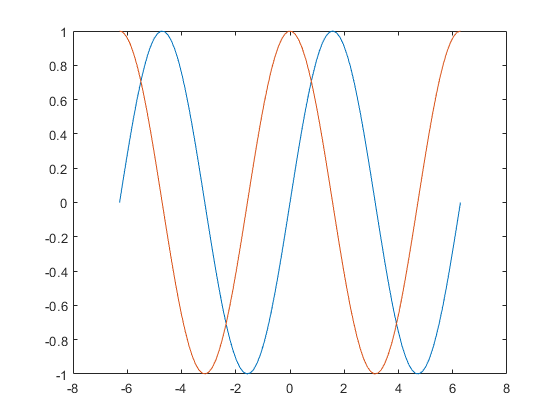
\includegraphics[width=0.75\textwidth]{plot.png}
    \caption{MatlabPlot}
    \label{fig:MatlabPlot}
\end{figure}

\subsection{Querverweise}
\label{sec:Querverweise}
Querverweis zu Kapitel \ref{sec:ZweiterAbschnitt}, Querverweis zu Tabelle \ref{tab:Parameters}, Querverweis zu Abbildung \ref{fig:MatlabPlot} und Querverweis zu Formel \eqref{eq:BrownianMotion}.
	
% Bibliography
	\newpage
	\printbibliography
	
% Appendix (comment out if not necessary)
	\newpage
	\appendix % Enumerates appendix with letters.
	\section{Appendix}

\begin{table}[H]
    \centering
    \begin{threeparttable}
    \begin{tabular}{@{}lllllll@{}}
        \toprule
        Feature Name            & Definition                                                                                       & Origin               & FS 1 & FS 2 & FS 3 & Transform     \\ \midrule
        trade price             & $P_{i, t}$                                                                                       & tick rule            & x    & x    & x    & $\log(\cdot)$ \\
        price lag (ex)          & $P_{i, t-1}^{\text{ex}}$\tnote{*}                                                                & tick rule            & x    & x    & x    & $\log(\cdot)$ \\
        price lag (all)         & $P_{i, t-1}^{\text{all}}$\tnote{*}                                                               & tick rule            & x    & x    & x    & $\log(\cdot)$ \\
        price change lag (ex)   & $P_{i, t-1}^{\text{ex}}/P_{i, t}^{\text{ex}}$\tnote{*}                                           & tick rule            & x    & x    & x    &               \\
        price change lag (all)  & $P_{i, t-1}^{\text{all}}/P_{i, t}^{\text{all}}$\tnote{*}                                         & tick rule            & x    & x    & x    &               \\
        priced lead (ex)        & $P_{i, t+1}^{\text{ex}}$\tnote{*}                                                                & rev. tick rule       & x    & x    & x    & $\log(\cdot)$ \\
        price lead (all)        & $P_{i, t+1}^{\text{all}}$\tnote{*}                                                               & rev. tick rule       & x    & x    & x    & $\log(\cdot)$ \\
        price change lead (ex)  & $P_{i, t}^{\text{ex}}/P_{i, t+1}^{\text{ex}}$\tnote{*}                                           & rev. tick rule       & x    & x    & x    &               \\
        price change lead (all) & $P_{i, t}^{\text{all}}/P_{i, t+1}^{\text{all}}$\tnote{*}                                         & rev. tick rule       & x    & x    & x    &               \\
        bid (all)               & $B_{i, t}^{\text{all}}$                                                                          & quote rule           & x    & x    & x    & $\log(\cdot)$ \\
        bid (ex)                & $B_{i, t}^{\text{ex}}$                                                                           & quote rule           & x    & x    & x    & $\log(\cdot)$ \\
        ask (all)               & $A_{i, t}^{\text{all}}$                                                                          & quote rule           & x    & x    & x    & $\log(\cdot)$ \\
        ask (ex)                & $A_{i, t}^{\text{all}}$                                                                          & quote rule           & x    & x    & x    & $\log(\cdot)$ \\
        prox. to quotes (ex)    & $\left(P_{i, t}^{\text{ex}}- M_{i, t}^{\text{ex}}\right) / \tfrac{1}{2} S_{i, t}^{\text{ex}}$    & \gls{EMO}/\gls{CLNV} & x    & x    & x    &               \\
        prox. to quotes (all)   & $\left(P_{i, t}^{\text{all}}- M_{i, t}^{\text{all}}\right) / \tfrac{1}{2} S_{i, t}^{\text{all}}$ & \gls{EMO}/\gls{CLNV} & x    & x    & x    &               \\
        bid ask size ratio (ex) & $\tilde{B}_{i, t}^{\text{ex}}/\tilde{A}_{i, t}^{\text{ex}}$                                      & depth rule           &      & x    & x    &               \\
        bid size (ex)           & $\tilde{B}_{i, t}^{\text{ex}}$                                                                   & depth rule           &      & x    & x    &               \\
        ask size (ex)           & $\tilde{A}_{i, t}^{\text{ex}}$                                                                   & depth rule           &      & x    & x    &               \\
        rel. bid size (ex)      & $\tilde{B}_{i, t}^{\text{ex}}/\tilde{P}_{i, t}^{\text{ex}}$                                      & trade size rule      &      & x    & x    &               \\
        rel. ask size (ex)      & $\tilde{A}_{i, t}^{\text{ex}}/\tilde{P}_{i, t}^{\text{ex}}$                                      & trade size rule      &      & x    & x    &               \\
        trade size              & $\tilde{P}_{i, t}$                                                                               & trade size rule      &      & x    & x    &               \\
        strike price            &                                                                                                  & option               &      &      & x    & $\log(\cdot)$ \\
        volume option series    &                                                                                                  & option               &      &      & x    & $\log(\cdot)$ \\
        root                    &                                                                                                  & option               &      &      & x    & binarize      \\
        time to maturity        &                                                                                                  & option               &      &      & x    &               \\
        moneyness               &                                                                                                  & option               &      &      & x    &               \\
        option type             &                                                                                                  & option               &      &      & x    & binarize      \\
        issue type              &                                                                                                  & option               &      &      & x    & binarize      \\ \bottomrule
    \end{tabular}
    \begin{tablenotes}\footnotesize
        \item[*] Notation assumes, that the previous or next trade price is distinguishable.
    \end{tablenotes}
\end{threeparttable}
    \caption[Feature Set Definition]{Feature Set Definition}
    \label{tab:feature-set-definition}
\end{table}
	
% Declaration 
	\newpage\thispagestyle{empty}
%	
% Declaration for Bachelor Thesis or Master Thesis

\begin{center}
{\LARGE {\textbf{Declaration}}}\\[2.5cm]
\end{center}
I truthfully declare that I have written the thesis
\vspace{1cm}
\begin{center}
\large {\titleofthesis}\\
\vspace{1cm}
\end{center}
independently, that I have completely and accurately indicated all sources and aids used, and that I have marked everything that has been taken unchanged or with modifications from the work of others, and that I have observed the KIT Statutes for Safeguarding Good Scientific Practice in the currently valid version.\\[2.5cm]
{\city}, {\dateofthesis}\\[0.75cm]
\hspace*{9.0cm}.....................................................\\
\hspace*{11.1cm}\name


 % Exclude title page (with %) that is not being used.
	
% Declaration for Seminar Thesis

\begin{center}
{\LARGE {\textbf{Declaration}}}\\[2.5cm]
\end{center}
I declare truthfully that I have written the thesis
\vspace{1cm}
\begin{center}
\large {\titleofthesis}\\
\vspace{1cm}
\end{center}
independently, that I have indicated all aids used completely and accurately, and that I have and to have marked everything that has been taken from the work of others unchanged or with modifications from the work of others.\\[2.5cm]
{\city}, {\dateofthesis}\\[0.75cm]
\hspace*{9.0cm}.....................................................\\
\hspace*{11.1cm}\name




\end{document}